\chapter{Superficies compactas}

\section{Superfies topológicas}

En primer lugar recordaremos algunos conceptos de Topología I para poder definir los nuevos conceptos de esta sección.

\begin{definicion}
    Diremos que un espacio topológico $X$ es T2 (o de \textbf{Haussforff}, o que satisface el \textbf{segundo axioma de separación}) si $\forall x,y \in X$ existe un abierto $U$ que contenga a $x$ y un abierto $V$ que contenga a $y$ tal que $U\cap V = \emptyset$.
        
        \begin{center}
            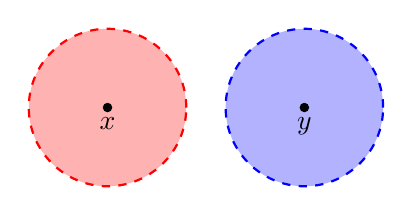
\begin{tikzpicture}
                \centering
    
                \def\radius{1}
    
                % Desactiva los caracteres conflictivos
                \shorthandoff{>} % Para poner puntas de flecha
    
                % Background
                \filldraw[thick, dashed, red, fill=red!30] (-1,0) circle (\radius);
                \filldraw[thick, dashed, blue, fill=blue!30] (1.5,0) circle (\radius);
    
                \filldraw (-1,0) circle (1.5pt) node[below] {$x$};
                \filldraw (1.5,0) circle (1.5pt) node[below] {$y$};
    
            \end{tikzpicture}
        \end{center}
\end{definicion}

\begin{definicion}
    Decimos que un espacio topológico $X$ es 2AN (o que cumple el \textbf{segundo axioma de numerabilidad}) si existe una base de la topología numerable.
\end{definicion}

Una vez recordados estos conceptos pasamos a las nuevas definiciones de esta sección:

\begin{definicion}
    Decimos que un espacio topológico $X$ es \textbf{localmente euclídeo} si para cada $x\in X$ existe un entorno abierto suyo que es homeomorfo a un abierto de $\bb{R}^n$.
\end{definicion}

\begin{definicion}
    Decimos que $S$ es una \textbf{superficie} si $S$ es un espacio topológico tal que $\forall x \in S$ existe un abierto que contiene a $x$ y que es homeomorfo a un abierto de $\bb{R}^2$. Además, pediremos que $S$ sea T2 (o Hausdorff) y 2AN (segundo axioma de numerabilidad).
\end{definicion}

\begin{ejemplo}\
    \begin{enumerate}
        \item $\bb{R}^2$ y $\bb{S}^2$ son superficies.
        \begin{proof}
            En el caso de $\bb{R}^2$ es trivial ya que para cualquier punto $x\in \bb{R}^2$ podemos considerar el total, $\bb{R}^2$ que es abierto, contiene a $x$ y es homeomorfo a sí mismo.\\

            En el caso de $\bb{S}^2$ podemos considerar para cada $x\in \bb{S}^2$ el conjunto $A = \bb{S}^2\setminus\{-x\}$, es decir, la esfera quitándole la antípoda. Sabemos que $A$ es abierto (ya que su complementario es $\{-x\}$ que es cerrado) y que contiene a $x$ (ya que $0\notin \bb{S}^2$). Además sabemos que $A$ es homeomorfo a $\bb{R}^2$ que es un abierto de $\bb{R}^2$ (el total).
        \end{proof}
        \item Cualquier abierto de una superficie es también una superficie. En particular, las bolas abiertas de $\bb{R}^2$ son también superficies.
        \begin{proof}
            Consideramos $A$ el abierto de la superficie $S$ y un punto cualquiera $x\in A$. Por ser $S$ una superficie existe un abierto $U$ que contiene a $x$ y que es homeomorfo (por $h$) a un abierto de $\bb{R}^2$. Consideramos entonces $A\cap U$ que es abierto por ser intersección de dos abiertos y que además contiene a $x$. Podemos considerar la restricción en el dominio del homeomorfismo $h$ a $A\cap U$ que seguirá siendo un homeomorfismo a un abierto de $\bb{R}^2$. Como esto se verifica para todo $x\in A$ tendremos que $A$ es una superficie.
        \end{proof}
        \item Sea $X=\{x\in \bb{R}^2 : \|x\|\leq r\} = \overline{B}(0,r)$. Entonces $X$ no es una superficie porque para los puntos $x$ con $\|x\| = r$ no existe un entorno abierto que lo contenga y que sea homeomorfo a un abierto de $\bb{R}^2$.
        \begin{proof}
            Tomamos un punto $x\in X$ con $\|x\|=r$. Si existiese $U$ entorno abierto suyo homeomorfo a un abierto $A$ de $\bb{R}^2$ entonces $\exists V$ entorno abierto de $x$ contenido en $U$ que es de la forma $V=B(x,r_0)\cap X$. Entonces $V$ es homeomorfo a un abierto $A'$ de $\bb{R}^2$ (ya que sería una restricción en el dominio del homeomorfismo entre $h:U\to A$). De esta forma tendríamos que como $V\setminus \{x\}$ es convexo debe ser simplemente conexo. Sin embargo, su imagen por homeomorfismo $h$ será $A'\setminus \{h(x)\}$ y como $h(x)$ está en el abierto $A'$ existe un radio $r_0'>0$ tal que $\overline{B}(h(x),r_0') \subseteq A'$. Pero el lazo dado por la frontera de dicha bola, $Fr(\overline{B}(h(x)r_0'))$ no es homotópicamente constante en $\bb{R}^2\setminus \{h(x)\}$. Por tanto este lazo no es homotópicamente constante en $A'\setminus\{h(x)\}$ por lo que $A'\setminus\{h(x)\}$ no es simplemente conexo. Esto prueba que $\overline{B}(0,r)$ no es una superficie.
        \end{proof}

        \item $\bb{S}^1\times \bb{R}$ y $\bb{S}^1\times \bb{S}^1$ son ejemplos de superficies. Esto se debe a que su recubridor universal es $\bb{R}^2$ luego sus aplicaciones recubridoras nos dan homeomorfismos locales desde abiertos de $\bb{R}^2$ en abiertos regularmente recubiertos de $\bb{S}^1 \times \bb{R}$ o $\bb{S}^1\times \bb{S}^1$.
    \end{enumerate}
\end{ejemplo}

\begin{observacion}
    Si $X$ es un espacio topológico localmente euclídeo entonces cumple las propiedades locales de $\bb{R}^n$. Por ejemplo, tiene una base de entornos numerable (es 1AN) y es localmente simplemente conexo. En particular, $X$ ha de tener recubridor universal.
\end{observacion}

\begin{definicion}
    Sea $S$ una superficie\footnote{siempre se entiende que es una superficie topológica} y $D$ un abierto dentro de $S$. Decimos que $D$ es un \textbf{disco regular} en $S$ si existe un abierto $D'$ tal que $D\subsetneq D'$ y un homeomorfismo $h:D'\to \bb{D}=\{x\in \bb{R}^2 : \|x\|<1\}=B((0,0),1)$ tal que $h(D)=\bb{D}_r=\{x\in \bb{R}^2 : \|x\|<r\}=B((0,0),r)$ con $0<r<1$.
\end{definicion}

\begin{ejemplo}\
    \begin{enumerate}
        \item Consideramos en $\bb{S}^2$:
        \begin{gather*}
            D = \{(x,y,z)\in \bb{S}^2 : z<r\} \text{ con } -1<r<1
        \end{gather*}
        En efecto es un disco regular. 
        \begin{proof}
            Como $-1<r<1$ tenemos que existe un $\veps >0$ tal que $r + \veps < 1$. Podemos fijar dicho $\veps$ y consideramos el siguiente conjunto
            \begin{gather*}
                D' = \{(x,y,z)\in \bb{S}^2 : z<r+\veps = r'\} \text{ con } -1<r'<1
            \end{gather*}
            En efecto tendremos que para cualquier punto $(x,y,z)\in D$ se tiene que $z<r<r'$ luego $(x,y,z)\in D'$. Además podemos considerar un punto $(x,y,z)\in \bb{S}^2$ tal que $z=r$ y tendremos que dicho punto está en $D'\setminus D$. Podemos concluir que $D\subsetneq D'$.

            \begin{figure}[H]
                \centering
                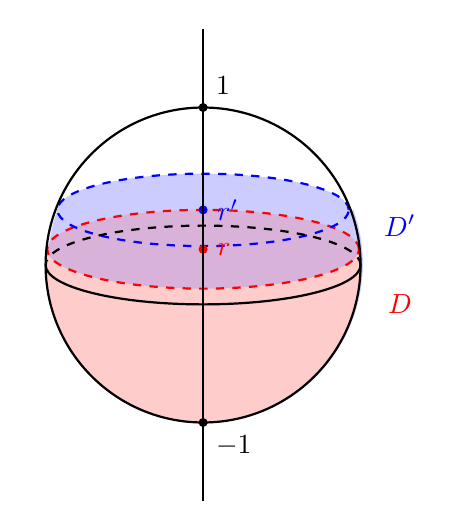
\begin{tikzpicture}
                    \shorthandoff{>}
                    \begin{scope}
                        % D y D'
                        \fill[blue!20] (-1.85, 0.7) arc (-200:20:2 and 2);
                        \fill[blue!20] (0,0.7) ellipse (1.85 and 0.46);

                        \fill[red!20] (-2,0.2) arc (-186:6:2 and 2);

                        \filldraw[thick, draw=red, fill=red!50!blue!30, dashed] (0,0.2) ellipse (1.98 and 0.5);

                        \draw[thick, blue, dashed] (0,0.7) ellipse (1.85 and 0.46);

                        \node[blue] at (2.5,0.5) {$D'$};
                        \node[red] at (2.5,-0.5) {$D$};

                        % r y r'
                        \node[draw, circle, red, fill=red, inner sep=1pt, label={[red]right:$r$}] at (0,0.2) {};
                        \node[draw, circle, blue, fill=blue, inner sep=1pt, label={[blue]right:$r'$}] at (0,0.7) {};

                        % Ejes
                        \draw[thick] (0,-3) -- (0,3);
                        \node[draw, circle, fill=black, inner sep=1pt, label=above right:$1$] at (0,2) {};
                        \node[draw, circle, fill=black, inner sep=1pt, label=below right:$-1$] at (0,-2) {};

                        % Esfera
                        \draw[thick] (0,0) circle [radius=2];
                        \draw[thick, dashed] (2,0) arc (0:180:2 and 0.5);
                        \draw[thick] (2,0) arc (0:-180:2 and 0.5);
                    \end{scope}
                \end{tikzpicture}
            \end{figure}
            
            Buscamos ahora un homeomorfismo $h:D'\to \bb{D}$ tal que $h(D)=\bb{D}_s$ con $0<s<1$. Pensamos en la proyección estereográfica desde el polo norte, $h:D'\to \bb{\bb{R}}^2$. Gráficamente lo podemos ver de la siguiente forma:

            \begin{figure}[H]
                \centering
                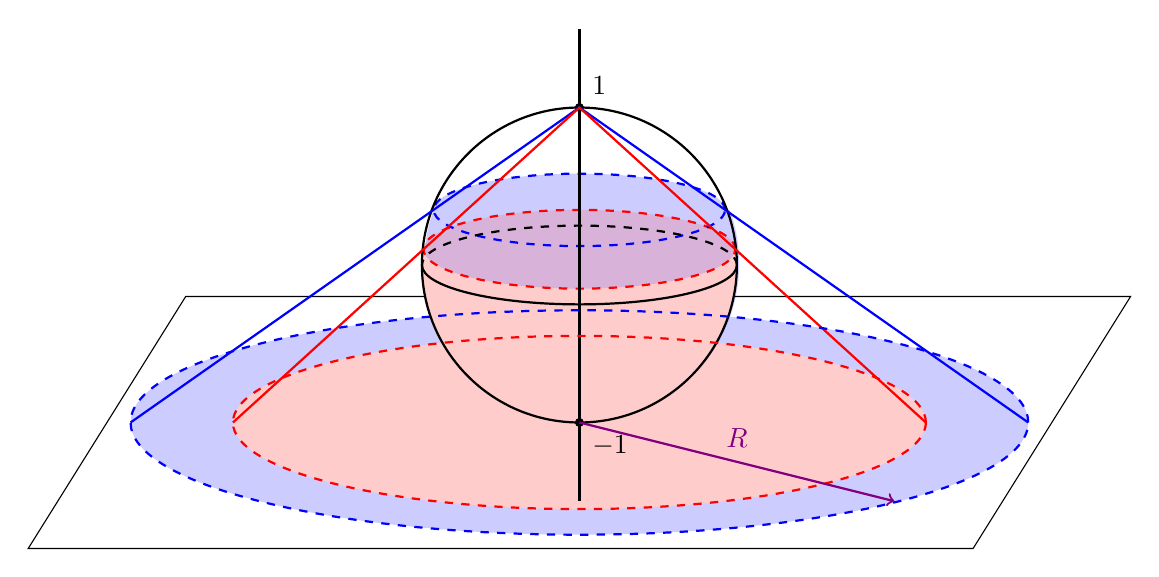
\begin{tikzpicture}
                    \shorthandoff{>}
                    \begin{scope}

                        \fill[thick, blue!20, dashed] (0,-2) ellipse (5.7 and 1.425);
                        \fill[thick, red!20, dashed] (0,-2) ellipse (4.4 and 1.1);

                        % D y D'
                        \fill[blue, opacity=0.2] (-1.85, 0.7) arc (-200:20:2 and 2);
                        \fill[blue!20] (0,0.7) ellipse (1.85 and 0.46);

                        \fill[red!20] (-2,0.2) arc (-186:6:2 and 2);

                        \filldraw[thick, draw=red, fill=red!50!blue!30, dashed] (0,0.2) ellipse (1.98 and 0.5);

                        \draw[thick, blue, dashed] (0,0.7) ellipse (1.85 and 0.46);

                        % Ejes
                        \draw[thick] (0,-3) -- (0,3);
                        \node[draw, circle, fill=black, inner sep=1pt, label=above right:$1$] at (0,2) {};
                        \node[draw, circle, fill=black, inner sep=1pt, label=below right:$-1$] at (0,-2) {};

                        % Esfera
                        \draw[thick] (0,0) circle [radius=2];
                        \draw[thick, dashed] (2,0) arc (0:180:2 and 0.5);
                        \draw[thick] (2,0) arc (0:-180:2 and 0.5);

                        % Plano suelo 
                        \draw (-1.95,-0.4) -- (-5, -0.4) -- (-7,-3.6) -- (5,-3.6) -- (7, -0.4) -- (1.95,-0.4);

                        \draw[thick, blue] (5.7 , -2) -- (0,2) -- (-5.7 , -2);
                        \draw[thick, red] (4.4 , -2) -- (0,2) -- (-4.4 , -2);
                        
                        \draw[thick, red, dashed] (0,-2) ellipse (4.4 and 1.1);
                        \draw[thick, blue, dashed] (0,-2) ellipse (5.7 and 1.425);

                        % Radio
                        \draw[thick, violet, ->] (0,-2) -- (4,-3);
                        \node[violet] at (2,-2.2) {$R$};
                    \end{scope}
                \end{tikzpicture}
            \end{figure}
        \end{proof}

        y llegamos a que existe un radio $R>0$ tal que podemos definir una nueva aplicación
        \Func{h'}{D'}{\bb{D}}{(x,y,z)}{\frac{1}{R}h(x,y,z)}
        que será un homeomorfismo (por serlo $h$). Además, es fácil ver que $h'(D) = \bb{D}_s$ con $0<s<1$.

        \item Consideramos la esfera sin el polo norte $D = \bb{S}^2\setminus \{(0,0,1)\}$ en $\bb{S}^2$. En este caso tendremos que no es un disco regular ya que el único abierto $D'$ que contiene estrictamente a $D$ es el total $D'=\bb{S}^2$ que sabemos que no es homeomorfo a ningún subconjunto de $\bb{R}^2$.

        \item $\bb{D}_r = B((0,0), r)\subseteq \bb{R}^2$ es un disco regular en $\bb{R}^2$ para todo $r\in \bb{R}^+$. Sin embargo, $\bb{D}_r$ no es regular en $S=\bb{D}_r$.
        
        \item En $\bb{R}^2$ consideramos el siguiente conjunto
        \begin{gather*}
            D=\bb{R}^2 \setminus \{(x,0) : x\geq 0\}
        \end{gather*}
        Entonces $D$ no puede ser un disco regular.
        \begin{proof}
            Si existiese un $D'$ que contiene a $D$ y contenido en $\bb{R}^2$ con $h: D' \to \bb{D}$ homeomorfismo tal que $h(D)= \bb{D}_r$ podemos tomar su restricción $h_{|D'\setminus D} : D'\setminus D  \to \bb{D}\setminus \bb{D}_r$ que seguirá siendo un homeomorfismo. Tenemos además que $D\subsetneq D \subseteq \bb{R}^2$ luego $D'\setminus D \subseteq \{(x,0) : x\geq 0\}$. Entonces tendremos que $(D'\setminus D)\setminus \{(x,0)\}$ no es convexo pero $h((D'\setminus D)\setminus \{(x,0)\}) = (\bb{D}\setminus \bb{D}_r)\setminus \{(h(x,0))\}$ es conexo por lo que no pueden ser homeomorfos y llegamos a contradicción.
        \end{proof}
    \end{enumerate}
\end{ejemplo}

\begin{lema}
    Sea $p_0$ un punto de una superficie $S$. Dado un entorno $U$ de $p_0$ existe $D$ disco regular que contiene a $p_0$ y está contenido en $U$. En particular, los discos regulares forman una base de la topología.
    \begin{proof}
        Como $S$ es una superficie, entonces para $p_0$ existe un abierto $V$ que contiene a $p_0$ y un homeomorfismo 
        \begin{gather*}
            \varphi : V \to \varphi(V)\subseteq \bb{R}^2
        \end{gather*}
        sobre $\varphi(V)$ que ha de ser abierto de $\bb{R}^2$. Ya que $\varphi(U\cap V)$ es un entorno de $\varphi(p_0)$ en $\bb{R}^2$ tenemos que existe un $R_0>0$ tal que
        \begin{gather*}
            B(\varphi(p_0), R_0)\subseteq \varphi(U\cap V)
        \end{gather*}
        Tomamos
        \begin{gather*}
            D=\varphi^{-1}\left(B\left(\varphi(p_0), \frac{R_0}{2}\right)\right)\\
            D'=\varphi^{-1}(B(\varphi(p_0), R_0))
        \end{gather*}
        Componiendo $\varphi$ con una transformación afín podemos llevar las bolas $B\left(\varphi(p_0), \frac{R_0}{2}\right)$ y $B(\varphi(p_0), R_0)$ a $\bb{D}_{\nicefrac{1}{2}}$ y $\bb{D}$ respectivamente.
    \end{proof}
\end{lema}

\begin{definicion}
    Sean $S_1$ y $S_2$ dos superficies conexas y disjuntas. Tomamos $D_1\subseteq S_1$ y $D_2\subseteq S_2$ discos regulares y consideramos un homeomorfismo $h: Fr(D_1)\to Fr(D_2)$. Sobre el espacio topológico $X=(S_1\setminus D_1)\cup (S_2\setminus D_2)$ consideramos la relación de equivalencia $R$ dada por
    \begin{gather*}
        x_1 R x_2 \sii \left\{
        \begin{array}{c}
            x_1=x_2\\
            \vee\\
            \{x_1,x_2\} = \{z, h(z)\} \text{ con } z\in Fr(D_1)
        \end{array}
        \right.
    \end{gather*}
    Denotamos por $S_1\# S_2$ al espacio topológico cociente de $X$ bajo la relación de equivalencia $R$ y lo llamaremos \textbf{suma conexa} de $S_1$ con $S_2$.
\end{definicion}

\begin{teo}
    El espacio topológico $S_1\#S_2$ es una superficie conexa que, salvo homeomorfismo, no depende de los discos $D_1$ y $D_2$ regulares ni del homeomorfismo $h$ entre sus fronteras.
\end{teo}

\begin{observacion}\
    \begin{enumerate}
        \item $S_1\#S_2 = S_2\#S_1$.

        \item Si $S_1$ es una superficie cualquiera y $S_2$ es la esfera $\bb{S}^2$, entonces 
        \begin{gather*}
            S_1\#S_2 = S_1\# \bb{S}^2 \cong S_1
        \end{gather*}
        % \begin{proof}
        %     Consideramos $D_1\subseteq S_1$ el disco regular de $S_1$ y $D_2\subseteq \bb{S}^2$ el disco regular de $\bb{S}^2$. Tenemos que $\bb{S}^2\setminus D_2$ es homeomorfo a un disco cerrado de $\bb{R}^2$. Pensamos ahora en el conjunto $\overline{D_1}$ que será homeomorfo a un disco cerrado de $\bb{S}^2$ y por tanto homeomorfo a $\bb{S}^2 \setminus D_2$. Si restringimos dicho homeomorfismo $h$ a la frontera tendremos que será un homeomorfismo $h_{|Fr(D_1)}:Fr(D_1) \to Fr(D_2)$ ya que $Fr(D_1) = Fr(\overline{D_1})$ y $Fr(D_2) = Fr(\bb{S}^2 \setminus D_2)$ y por tanto $S_1\#\bb{S}^2$ es homeomorfo a $S_1$ mediante $h$.
        % \end{proof}

        \item Si tenemos $n$ toros ($n\geq 2$) podemos definir 
        \begin{gather*}
            \bb{T}_n \equiv \text{suma conexa de los $n$ toros}
        \end{gather*}
        que recibe el nombre de \textbf{$n$-toro} o \textbf{esfera con $n$ asas}.

        \begin{figure}[H]
            \centering
            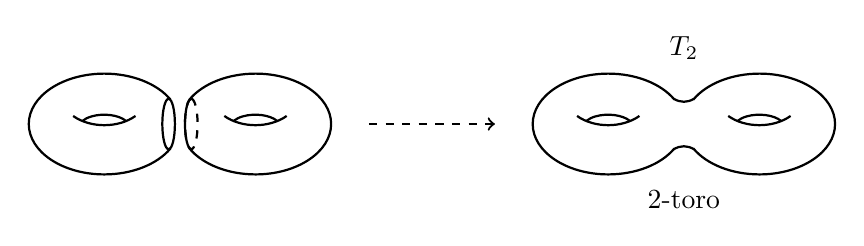
\begin{tikzpicture}[scale=0.8]
                \shorthandoff{>}
                \begin{scope}[scale=0.4, shift={(-10,0)}]
                    \begin{scope}[shift={(-3,0)}]
                        % Toro
                        % \draw[thick] (5,0) ellipse (3 and 2); % Exterior
                        \draw[thick] (-1.24,0.32) arc (225:315:1.75 and 1.25); % Agujero
                        \draw[thick] (0.86,0.12) arc (30:150:1 and 0.5);
                        % \draw[dashed] (5,0.2) ellipse (2.97 and 1.3); % Perímetro
                        \draw[thick] (-3,0) arc (-180:-29:3 and 2);
                        \draw[thick] (-3,0) arc (180:29:3 and 2);

                        % Boquete
                        \draw[thick] (2.55,0) ellipse (0.25 and 1); 
                    \end{scope}

                    \begin{scope}[shift={(3,0)}]
                        % Toro
                        % \draw[thick] (5,0) ellipse (3 and 2); % Exterior
                        \draw[thick] (-1.24,0.32) arc (225:315:1.75 and 1.25); % Agujero
                        \draw[thick] (0.86,0.12) arc (30:150:1 and 0.5);
                        % \draw[dashed] (5,0.2) ellipse (2.97 and 1.3); % Perímetro
                        \draw[thick] (3,0) arc (0:151:3 and 2);
                        \draw[thick] (3,0) arc (0:-151:3 and 2);

                        % Boquete
                        \draw[thick] (-2.55,1) arc (90:270:0.25 and 1);
                        \draw[thick, dashed] (-2.55,1) arc (90:-270:0.25 and 1);
                    \end{scope}
                \end{scope}

                \draw[thick, dashed, ->] (-1,0) -- (1,0);

                \begin{scope}[scale=0.4, shift={(10,0)}]
                    \begin{scope}[shift={(-3,0)}]
                        % Toro
                        % \draw[thick] (5,0) ellipse (3 and 2); % Exterior
                        \draw[thick] (-1.24,0.32) arc (225:315:1.75 and 1.25); % Agujero
                        \draw[thick] (0.86,0.12) arc (30:150:1 and 0.5);
                        % \draw[dashed] (5,0.2) ellipse (2.97 and 1.3); % Perímetro
                        \draw[thick] (-3,0) arc (-180:-29:3 and 2);
                        \draw[thick] (-3,0) arc (180:29:3 and 2); 
                    \end{scope}

                    \draw[thick, bend right=30] (-0.4,1) to (0.4,1);

                    \draw[thick, bend left=30] (-0.4,-1) to (0.4,-1);

                    \begin{scope}[shift={(3,0)}]
                        % Toro
                        % \draw[thick] (5,0) ellipse (3 and 2); % Exterior
                        \draw[thick] (-1.24,0.32) arc (225:315:1.75 and 1.25); % Agujero
                        \draw[thick] (0.86,0.12) arc (30:150:1 and 0.5);
                        % \draw[dashed] (5,0.2) ellipse (2.97 and 1.3); % Perímetro
                        \draw[thick] (3,0) arc (0:151:3 and 2);
                        \draw[thick] (3,0) arc (0:-151:3 and 2);

                    \end{scope}

                    \node at (0,3) {$\bb{T}_2$};
                    \node at (0, -3) {2-toro};
                \end{scope}
                
            \end{tikzpicture}
        \end{figure}
        \begin{figure}[H]
            \centering
            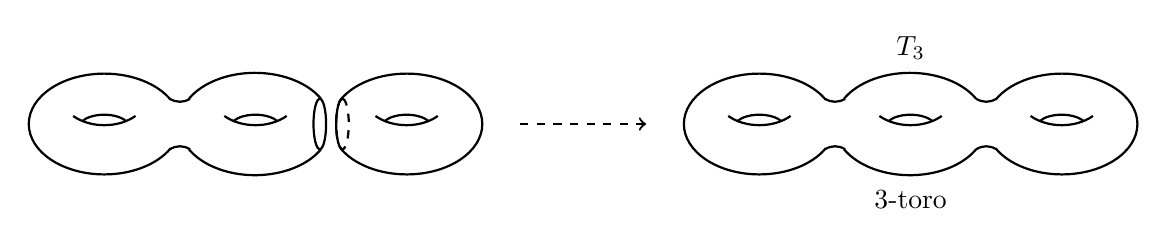
\begin{tikzpicture}[scale=0.8]
                \shorthandoff{>}
                \begin{scope}[scale=0.4, shift={(-16,0)}]
                    \begin{scope}[shift={(-3,0)}]
                        % Toro
                        % \draw[thick] (5,0) ellipse (3 and 2); % Exterior
                        \draw[thick] (-1.24,0.32) arc (225:315:1.75 and 1.25); % Agujero
                        \draw[thick] (0.86,0.12) arc (30:150:1 and 0.5);
                        % \draw[dashed] (5,0.2) ellipse (2.97 and 1.3); % Perímetro
                        \draw[thick] (-3,0) arc (-180:-29:3 and 2);
                        \draw[thick] (-3,0) arc (180:29:3 and 2); 
                    \end{scope}

                    \draw[thick, bend right=30] (-0.4,1) to (0.4,1);
                    \draw[thick, bend left=30] (-0.4,-1) to (0.4,-1);

                    \begin{scope}[shift={(3,0)}]
                        % Toro
                        \draw[thick] (-1.24,0.32) arc (225:315:1.75 and 1.25); % Agujero
                        \draw[thick] (0.86,0.12) arc (30:150:1 and 0.5);

                        % Exterior
                        \draw[thick] (2.6,1) arc (29:151:3 and 2);
                        \draw[thick] (2.6,-1) arc (-29:-151:3 and 2);

                        % Boquete
                        \draw[thick] (2.55,0) ellipse (0.25 and 1); 

                    \end{scope}

                    \begin{scope}[shift={(9,0)}]
                        % Toro
                        % \draw[thick] (5,0) ellipse (3 and 2); % Exterior
                        \draw[thick] (-1.24,0.32) arc (225:315:1.75 and 1.25); % Agujero
                        \draw[thick] (0.86,0.12) arc (30:150:1 and 0.5);
                        % \draw[dashed] (5,0.2) ellipse (2.97 and 1.3); % Perímetro
                        \draw[thick] (3,0) arc (0:151:3 and 2);
                        \draw[thick] (3,0) arc (0:-151:3 and 2);

                        % Boquete
                        \draw[thick] (-2.55,1) arc (90:270:0.25 and 1);
                        \draw[thick, dashed] (-2.55,1) arc (90:-270:0.25 and 1);

                    \end{scope}
                \end{scope}

                \draw[thick, dashed, ->] (-1,0) -- (1,0);

                \begin{scope}[scale=0.4, shift={(10,0)}]
                    \begin{scope}[shift={(-3,0)}]
                        % Toro
                        % \draw[thick] (5,0) ellipse (3 and 2); % Exterior
                        \draw[thick] (-1.24,0.32) arc (225:315:1.75 and 1.25); % Agujero
                        \draw[thick] (0.86,0.12) arc (30:150:1 and 0.5);
                        % \draw[dashed] (5,0.2) ellipse (2.97 and 1.3); % Perímetro
                        \draw[thick] (-3,0) arc (-180:-29:3 and 2);
                        \draw[thick] (-3,0) arc (180:29:3 and 2); 
                    \end{scope}

                    \draw[thick, bend right=30] (-0.4,1) to (0.4,1);
                    \draw[thick, bend left=30] (-0.4,-1) to (0.4,-1);

                    \begin{scope}[shift={(3,0)}]
                        % Toro
                        \draw[thick] (-1.24,0.32) arc (225:315:1.75 and 1.25); % Agujero
                        \draw[thick] (0.86,0.12) arc (30:150:1 and 0.5);

                        % Exterior
                        \draw[thick] (2.6,1) arc (29:151:3 and 2);
                        \draw[thick] (2.6,-1) arc (-29:-151:3 and 2);

                    \end{scope}

                    \node at (3,3) {$\bb{T}_3$};

                    \draw[thick, bend right=30] (5.6,1) to (6.4,1);
                    \draw[thick, bend left=30] (5.6,-1) to (6.4,-1);

                    \begin{scope}[shift={(9,0)}]
                        % Toro
                        % \draw[thick] (5,0) ellipse (3 and 2); % Exterior
                        \draw[thick] (-1.24,0.32) arc (225:315:1.75 and 1.25); % Agujero
                        \draw[thick] (0.86,0.12) arc (30:150:1 and 0.5);
                        % \draw[dashed] (5,0.2) ellipse (2.97 and 1.3); % Perímetro
                        \draw[thick] (3,0) arc (0:151:3 and 2);
                        \draw[thick] (3,0) arc (0:-151:3 and 2);
                    \end{scope}
                    \node at (3, -3) {3-toro};
                \end{scope}
                
            \end{tikzpicture}
        \end{figure}

        \item La suma conexa de $n$ planos proyectivos la llamaremos\footnote{no confundir con $\bb{R}\bb{P}^n$} \textbf{$n$ plano proyectivo}, $\bb{R}\bb{P}^2_n$.
    \end{enumerate}
\end{observacion}

\section{Presentaciones poligonales de superficies}

\begin{definicion}
    Consideramos el triángulo 
    \begin{gather*}
        T=\{(x,y)\in \bb{R}^2 : x\geq0,\ y\geq 0, x+y\leq 1\}
    \end{gather*}

    \begin{figure}[H]
        \centering
        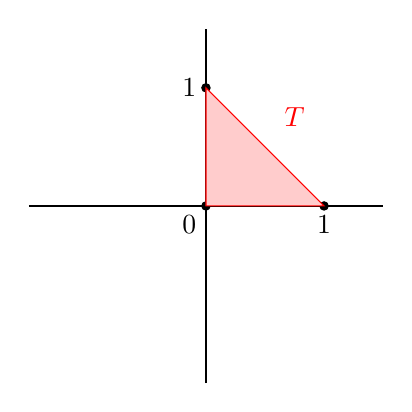
\begin{tikzpicture}[scale=1.5]
            \shorthandoff{>}
            % Ejes
            \draw[thick] (0,-1.5) -- (0,1.5);
            \draw[thick] (-1.5,0) -- (1.5,0);

            % Leyenda
            \filldraw (0,1) circle (1pt) node[left] {$1$};
            \filldraw (1,0) circle (1pt) node[below] {$1$};
            \filldraw (0,0) circle (1pt) node[below left] {$0$};
            \node[red] at (0.75,0.75) {$T$};

            \filldraw[draw=red, fill=red!20] (0,0) -- (1,0) -- (0,1) -- cycle;
        \end{tikzpicture}
    \end{figure}

    Decimos que un espacio topológico $X$ es un \textbf{triángulo} (topológico) si existe un homeomorfismo $h:T \to X$. En tal caso, llamaremos \textbf{vértices} de $X$ a la imagen mediante $h$ de los vértices de $T$ y \textbf{aristas} de $X$ a la imagen mediante $h$ de las aristas de $T$.
\end{definicion}

\begin{teo}[Teorema de Radó]
    Toda superficie compacta puede ser triangulada, es decir, la superficie puede verse como una unión finita triángulos (topológicos) de forma que dos triángulos distintos o bien son disjuntos o bien solo se intersecan en un vértice o solo en una arista.
\end{teo}

\begin{observacion}
    La idea de este teorema será que toda superficie compacta puede ser reconstruida pegando un número finito de triángulos a través de sus aristas.

    \begin{figure}[H]
        \centering
        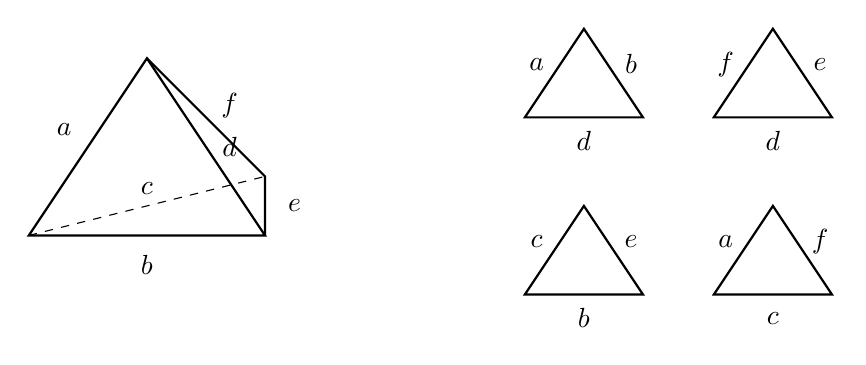
\begin{tikzpicture}[scale=1.5]
            \shorthandoff{>}
            \begin{scope}[shift={(0,0.5)}]
                % Pirámide
                \draw[thick] (0,0) -- (2,0) -- (1,1.5) -- cycle;
                \draw[thick] (2,0) -- (2,0.5) -- (1,1.5);
                \draw[dashed] (0,0) -- (2,0.5);

                % Leyenda
                \node at (0.3,0.9) {$a$};
                \node at (1,-0.25) {$b$};
                \node at (1,0.4) {$c$};
                \node at (1.7,0.75) {$d$};
                \node at (2.25,0.25) {$e$};
                \node at (1.7,1.1) {$f$};
            \end{scope}

            \begin{scope}[shift={(5,0)}]
                \begin{scope}[shift={(-0.8,1.5)}]
                    \draw[thick] (0,0) -- (1,0) -- (0.5,0.75) -- cycle;
                    % Leyenda
                    \node at (0.1,0.45) {$a$};
                    \node at (0.5,-0.2) {$d$};
                    \node at (0.9,0.45) {$b$};
                \end{scope}
                \begin{scope}[shift={(-0.8,0)}]
                    \draw[thick] (0,0) -- (1,0) -- (0.5,0.75) -- cycle;
                    % Leyenda
                    \node at (0.1,0.45) {$c$};
                    \node at (0.5,-0.2) {$b$};
                    \node at (0.9,0.45) {$e$};
                \end{scope}
                \begin{scope}[shift={(0.8,1.5)}]
                    \draw[thick] (0,0) -- (1,0) -- (0.5,0.75) -- cycle;
                    % Leyenda
                    \node at (0.1,0.45) {$f$};
                    \node at (0.5,-0.2) {$d$};
                    \node at (0.9,0.45) {$e$};
                \end{scope}
                \begin{scope}[shift={(0.8,0)}]
                    \draw[thick] (0,0) -- (1,0) -- (0.5,0.75) -- cycle;
                    % Leyenda
                    \node at (0.1,0.45) {$a$};
                    \node at (0.5,-0.2) {$c$};
                    \node at (0.9,0.45) {$f$};
                \end{scope}
            \end{scope}
        \end{tikzpicture}
    \end{figure}
\end{observacion}

\begin{definicion}
    Llamaremos presentación poligonal de una superficie compacta a una expresión de la forma 
    \begin{gather*}
        \cc{P} = \{a_1,...,a_n; w_1,...,w_m\} \text{ con } n,m\in \bb{N}
    \end{gather*}
    donde los $a_i$ son símbolos y los $w_j$ son expresiones del tipo
    \begin{gather*}
        w_i=a_{i1}^{\veps_{i1}}...a_{ik}^{\veps_{ik}}
    \end{gather*}
    donde $k\geq 3$ (es decir, hay al menos $3$ símbolos en la expresión $w_i$) y cada $\veps_{il}\in \{1,-1\}$ para cada $l\in\{1,...,k\}$. Y además, el número de veces que aparece cada símbolo en el total de los $w_i$ es $2$.
\end{definicion}

\begin{ejemplo}\
    \begin{enumerate}
        \item $\cc{P}=\{a,b;aba^{-1}b^{-1}\}$.
        \item $\cc{P}=\{a,b,c; aab, bcc^{-1}\}$.
        \item $\cc{P}=\{a,b,c,d; aab, bcd, cdd^{-1}\}$ no es una presentación ya que la $d$ aparece 3 veces.
    \end{enumerate}
\end{ejemplo}

\begin{definicion}
    A cada presentación poligonal $\cc{P}$ le asociaremos un espacio toloógico que denotaremos por $|\cc{P}|$ y que llamaremos la \textbf{realización geométrica de la presentación poligonal}. Su construcción es la siguiente
    \begin{enumerate}
        \item Para cada $w_i$ consideramos un polígono $P_i$ (regular) con número de lados igual al número de símbolos de $w_i$. Los $P_i$ serán disjuntos entre sí.
        \item Para cada $P_i$ asociado a un $w_i$ elegimos un lado cualquiera y en sentido contrario de las agujas del reloj, nombramos cada lado de $P_i$ con el nombre del símbolo. Además a cada lado le daremos la orientación contraria a las agujas del reloj si el exponente es $1$ y la orientación contraria si el exponente es $-1$.
        \item En el espacio topológico dado por la unión de todos los polígonos $P_i$ consideramos la relación la equivalencia que identifica los lados con igual nombre mediante el único homeomorfismo (aplicación que lleva un lado en otro sin cambiar el sentido de las flechas).
        \item Llamamos $|\cc{P}|$ al espacio cociente dado por la unión de los polígonos bajo la relación de equivalencia anterior.
    \end{enumerate}
\end{definicion}

\begin{ejemplo}
    $\cc{P}=\{a,b,c,d; abc^{-1}d, a^{-1}b^{-1}cd^{-1}\}$
    \begin{enumerate}
        \item \
        \begin{figure}[H]
            \centering
            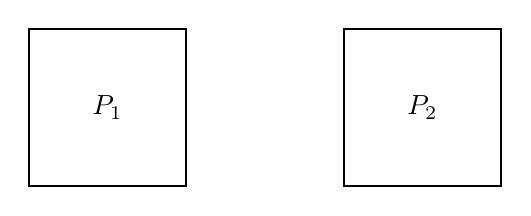
\begin{tikzpicture}
                \shorthandoff{>}
                \begin{scope}
                    \draw[thick] (-1,-1) -- (1,-1) -- (1,1) -- (-1,1) -- cycle;
                    \node at (0,0) {$P_1$};
                \end{scope}
                \begin{scope}[shift={(4,0)}]
                    \draw[thick] (-1,-1) -- (1,-1) -- (1,1) -- (-1,1) -- cycle;
                    \node at (0,0) {$P_2$};
                \end{scope}
            \end{tikzpicture}
        \end{figure}

        \item \
        \begin{figure}[H]
            \centering
            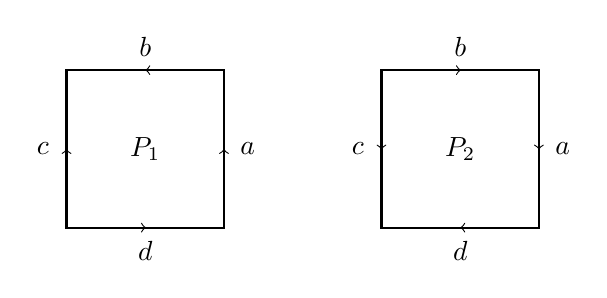
\begin{tikzpicture}
                \shorthandoff{>}
                \begin{scope}
                    \draw[thick] (-1,-1) -- (1,-1) -- (1,1) -- (-1,1) -- cycle;
                    \node at (0,0) {$P_1$};

                    % Aristas
                    \node at (1.3,0) {$a$};
                    \node at (0,1.3) {$b$};
                    \node at (-1.3,0) {$c$};
                    \node at (0,-1.3) {$d$};

                    %Sentidos
                    \draw[->] (1,0) ++(0, -0.01) -- ++(0,0.01); %a
                    \draw[->] (0,1) ++(0.01, 0) -- ++(-0.01,0); %b
                    \draw[->] (-1,0) ++(0, -0.01) -- ++(0,0.01); %c
                    \draw[<-] (0,-1) ++(0.01, 0) -- ++(-0.01,0); %d

                \end{scope}
                \begin{scope}[shift={(4,0)}]
                    \draw[thick] (-1,-1) -- (1,-1) -- (1,1) -- (-1,1) -- cycle;
                    \node at (0,0) {$P_2$};

                    % Aristas
                    \node at (1.3,0) {$a$};
                    \node at (0,1.3) {$b$};
                    \node at (-1.3,0) {$c$};
                    \node at (0,-1.3) {$d$};

                    %Sentidos
                    \draw[<-] (1,0) ++(0, -0.01) -- ++(0,0.01); %a
                    \draw[<-] (0,1) ++(0.01, 0) -- ++(-0.01,0); %b
                    \draw[<-] (-1,0) ++(0, -0.01) -- ++(0,0.01); %c
                    \draw[->] (0,-1) ++(0.01, 0) -- ++(-0.01,0); %d
                \end{scope}
            \end{tikzpicture}
        \end{figure}

        \item \
        \begin{figure}[H]
            \centering
            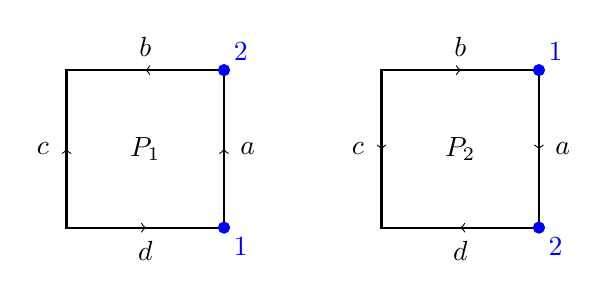
\begin{tikzpicture}
                \shorthandoff{>}
                \begin{scope}
                    \draw[thick] (-1,-1) -- (1,-1) -- (1,1) -- (-1,1) -- cycle;
                    \node at (0,0) {$P_1$};

                    % Aristas
                    \node at (1.3,0) {$a$};
                    \node at (0,1.3) {$b$};
                    \node at (-1.3,0) {$c$};
                    \node at (0,-1.3) {$d$};

                    %Sentidos
                    \draw[->] (1,0) ++(0, -0.01) -- ++(0,0.01); %a
                    \draw[->] (0,1) ++(0.01, 0) -- ++(-0.01,0); %b
                    \draw[->] (-1,0) ++(0, -0.01) -- ++(0,0.01); %c
                    \draw[<-] (0,-1) ++(0.01, 0) -- ++(-0.01,0); %d

                    %Identificaciones
                    \filldraw[blue] (1,1) circle (2pt) node[above right] {$2$};
                    \filldraw[blue] (1,-1) circle (2pt) node[below right] {$1$};
                \end{scope}
                \begin{scope}[shift={(4,0)}]
                    \draw[thick] (-1,-1) -- (1,-1) -- (1,1) -- (-1,1) -- cycle;
                    \node at (0,0) {$P_2$};

                    % Aristas
                    \node at (1.3,0) {$a$};
                    \node at (0,1.3) {$b$};
                    \node at (-1.3,0) {$c$};
                    \node at (0,-1.3) {$d$};

                    %Sentidos
                    \draw[<-] (1,0) ++(0, -0.01) -- ++(0,0.01); %a
                    \draw[<-] (0,1) ++(0.01, 0) -- ++(-0.01,0); %b
                    \draw[<-] (-1,0) ++(0, -0.01) -- ++(0,0.01); %c
                    \draw[->] (0,-1) ++(0.01, 0) -- ++(-0.01,0); %d

                    % Identificaciones 
                    \filldraw[blue] (1,1) circle (2pt) node[above right] {$1$};
                    \filldraw[blue] (1,-1) circle (2pt) node[below right] {$2$};
                \end{scope}
            \end{tikzpicture}
        \end{figure}
    \end{enumerate}
\end{ejemplo}

\begin{ejemplo}\
    \begin{figure}[H]
        \centering
        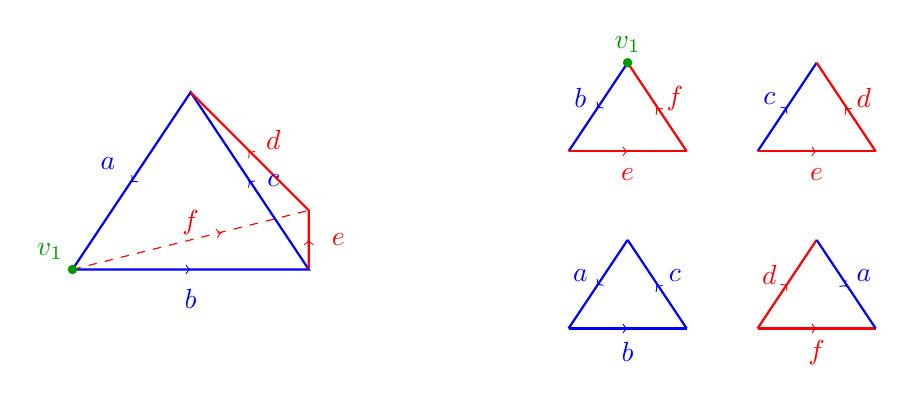
\begin{tikzpicture}[scale=1.5]
            \shorthandoff{>}
            \begin{scope}[shift={(0,0.5)}]
                % Pirámide
                \draw[thick, blue] (0,0) -- (2,0) -- (1,1.5) -- cycle;
                \draw[thick, red] (2,0) -- (2,0.5) -- (1,1.5);
                \draw[dashed, red] (0,0) -- (2,0.5);

                % Leyenda
                \node[blue] at (0.3,0.9) {$a$};
                \node[blue] at (1,-0.25) {$b$};
                \node[red] at (1,0.4) {$f$};
                \node[blue] at (1.7,0.75) {$c$};
                \node[red] at (2.25,0.25) {$e$};
                \node[red] at (1.7,1.1) {$d$};

                % Flechas
                \draw[<-, blue] (0.5,0.75) ++(0, -0.01) -- ++(0.01,0.01); %a
                \draw[->, blue] (1,0) ++(-0.01,0) -- ++(0.01,0); %b
                \draw[->, blue] (1.5,0.75) ++(0, -0.01) -- ++(-0.01,0.01); %c
                \draw[->, red] (1.5,1) ++(0, -0.01) -- ++(-0.01,0.01); %d
                \draw[->, red] (2,0.25) ++(0, -0.01) -- ++(0,0.01); %e
                \draw[->, red] (1.25,0.32) ++(0, -0.01) -- ++(0.01,0.002); %f

                % Identificaciones
                \filldraw[green!60!black] (0,0) circle (1pt) node[above left] {$v_1$};
            \end{scope}

            \begin{scope}[shift={(5,0)}]
                \begin{scope}[shift={(-0.8,1.5)}]
                    % Triángulo
                    \draw[thick, blue] (0.5,0.75) -- (0,0); %1
                    \draw[thick, red] (0,0) -- (1,0); %2
                    \draw[thick, red] (1,0) -- (0.5,0.75); %3

                    % Leyenda
                    \node[blue] at (0.1,0.45) {$b$};
                    \node[red] at (0.5,-0.2) {$e$};
                    \node[red] at (0.9,0.45) {$f$};

                    % Flechas
                    \draw[->, blue] (0.25,0.365) ++(0, 0.01) -- ++(-0.01,-0.01); %1
                    \draw[->, red] (0.5,0) ++(-0.01,0) -- ++(0.01,0); %2
                    \draw[->, red] (0.75,0.365) ++(0, -0.01) -- ++(-0.01,0.01); %3

                    % Identificación
                    \filldraw[green!60!black] (0.5,0.75) circle (1pt) node[above] {$v_1$};
                \end{scope}
                \begin{scope}[shift={(-0.8,0)}]
                    % Triángulo
                    \draw[thick, blue] (0.5,0.75) -- (0,0); %1
                    \draw[thick, blue] (0,0) -- (1,0); %2
                    \draw[thick, blue] (1,0) -- (0.5,0.75); %3

                    % Leyenda
                    \node[blue] at (0.1,0.45) {$a$};
                    \node[blue] at (0.5,-0.2) {$b$};
                    \node[blue] at (0.9,0.45) {$c$};

                    % Flechas
                    \draw[->, blue] (0.25,0.365) ++(0, 0.01) -- ++(-0.01,-0.01); %1
                    \draw[->, blue] (0.5,0) ++(-0.01,0) -- ++(0.01,0); %2
                    \draw[->, blue] (0.75,0.365) ++(0, -0.01) -- ++(-0.01,0.01); %3
                \end{scope}
                \begin{scope}[shift={(0.8,1.5)}]
                    % Triángulo
                    \draw[thick, blue] (0.5,0.75) -- (0,0); %1
                    \draw[thick, red] (0,0) -- (1,0); %2
                    \draw[thick, red] (1,0) -- (0.5,0.75); %3

                    % Leyenda
                    \node[blue] at (0.1,0.45) {$c$};
                    \node[red] at (0.5,-0.2) {$e$};
                    \node[red] at (0.9,0.45) {$d$};

                    % Flechas
                    \draw[<-, blue] (0.25,0.365) ++(0, 0.01) -- ++(-0.01,-0.01); %1
                    \draw[->, red] (0.5,0) ++(-0.01,0) -- ++(0.01,0); %2
                    \draw[->, red] (0.75,0.365) ++(0, -0.01) -- ++(-0.01,0.01); %3
                \end{scope}
                \begin{scope}[shift={(0.8,0)}]
                    % Triángulo
                    \draw[thick, red] (0.5,0.75) -- (0,0); %1
                    \draw[thick, red] (0,0) -- (1,0); %2
                    \draw[thick, blue] (1,0) -- (0.5,0.75); %3

                    % Leyenda
                    \node[red] at (0.1,0.45) {$d$};
                    \node[red] at (0.5,-0.2) {$f$};
                    \node[blue] at (0.9,0.45) {$a$};

                    % Flechas
                    \draw[<-, red] (0.25,0.365) ++(0, 0.01) -- ++(-0.01,-0.01); %1
                    \draw[->, red] (0.5,0) ++(-0.01,0) -- ++(0.01,0); %2
                    \draw[<-, blue] (0.75,0.365) ++(0, -0.01) -- ++(-0.01,0.01); %3
                \end{scope}
            \end{scope}
        \end{tikzpicture}
    \end{figure}
    Tendríamos entonces $\cc{P}=\{a,b,c,d; abc, c^{-1}ed, a^{-1}d^{-1}f, bef\}$
\end{ejemplo}
